\section{Results}
Like in the methods section, this section will also be in two parts. This is due to the two compression methods, that are to be tested, are so different in nature and cannot be directly compared. To compare the methods, the a set of metrics will be applied to the original and compressed models. The metrics are:
\begin{itemize}
    \item \textbf{Accuracy} - especially the accuracy drop is an important metric in comparing the compressed model to the full model
    \item \textbf{Number of Parameters} - how much space the model takes to store
    \item \textbf{Theoretical speed} - based on the number of FLOPs, calculated using the formulas given in \autoref{tex:computational_complexity}.
    \item \textbf{Actual speed} - how long it takes to compute a forward push. Computed many times reporting the mean and standard deviation of the time it takes
\end{itemize}
Initially the results of the method of decomposing the input will be given, followed by the results of decomposing a pre-trained network.

\subsection{Decomposing the Input}


\subsubsection{Experiment with low rank}
In the following an experiment is carried out to check whether the decomposition itself can carry much of the training. Since we have only 2 classes for the THETIS data set, and for the sake of the experiment 2 digits from the MNIST data set will be used. Since there are 2 classes in each data set, an initial rank of 2 will be experimentally chosen in the between sample dimension. The results for both the data set are described in the following.

\paragraph{Using MNIST 3s and 4s}
Only the MNIST observations depicting either a 3 or a 4 will be considered in this experiment. These digits are chosen due to their distinct shapes, hence ease of classification. Since the purpose is to make the algorithm find the differences between the two different digits, the spatial dimensions will not be decomposed. Using the experimental rank of 2, the decomposition of $N$ stacked 3s and 4s becomes:
\begin{equation}
    \tensor{X}^{N\times 28\times 28} \approx \tensor{G}^{2 \times 28 \times 28} \times_1 \bs{A}^{N\times 2} \qquad \Leftrightarrow \qquad \bs{X}_{(1)} \approx \bs{A}^{N\times 2} \ \bs{G}^{2 \times 28\cdot 28}_{(1)}
\end{equation}
Where $\bs{A}$ is the loading matrix in the dimension corresponding to different pictures. With the rank equal to 2, $\bs{A}$ holds 2 values per picture that should ideally be separating the two digits that is to be trained. \autoref{fig:decompExample3_4} shows how the decomposition of the first 100 training examples turns out. It seems the decomposition is able how to find the "general 3" and the "general 4", and then simply use the loadings of $\bs{A}$ to specify how much of each should be used to represent every observation. \autoref{fig:loadingAMatrix} shows a scatter-plot of the values of $\bs{A}$ colored to show the loadings corresponding to 3s and 4s respectively. There is some overlap between the two clusters, but it seems that they can be fairly distinguished. Using the mean of $\bs{A}$ of the the 3s, 4s and overall respectively as loadings in the decomposition yields the approximated pictures shown in \autoref{fig:loadingsOfA}b-d.

\begin{figure}
    \centering
    \begin{subfigure}{0.45\linewidth}
        \centering
        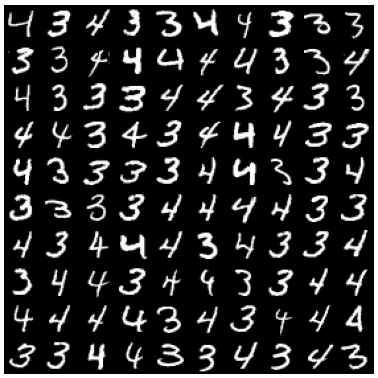
\includegraphics[width=\linewidth]{Pics/06_results/3_4_original.png}
        \captionsetup{width=.9\linewidth}
        \caption{Original MNIST training examples including only 3s and 4s.}
    \end{subfigure}
    \begin{subfigure}{0.45\linewidth}
        \centering
        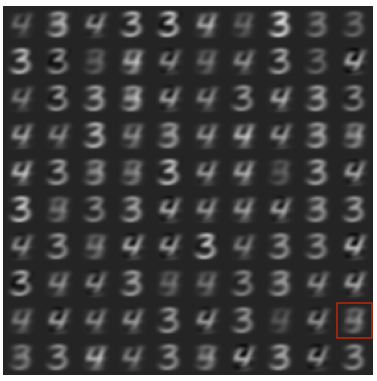
\includegraphics[width=\linewidth]{Pics/06_results/3_4_decomp.png}
        \captionsetup{width=.9\linewidth}
        \caption{Approximated versions of the training examples on the left, using the decomposition.}
    \end{subfigure}
    \captionsetup{width=.95\linewidth}
    \caption{MNIST training examples before and after decomposing with only rank 2 in the input dimension. Notice how the decomposed 3s and 4s look more standardized. It seems that every picture is a part standardized 3 and a part standardized 4. Notice how digits that look relatively odd results in less certain approximation.}
    \label{fig:decompExample3_4}
\end{figure}

\begin{figure}
    \centering
    \begin{subfigure}{0.99\linewidth}
        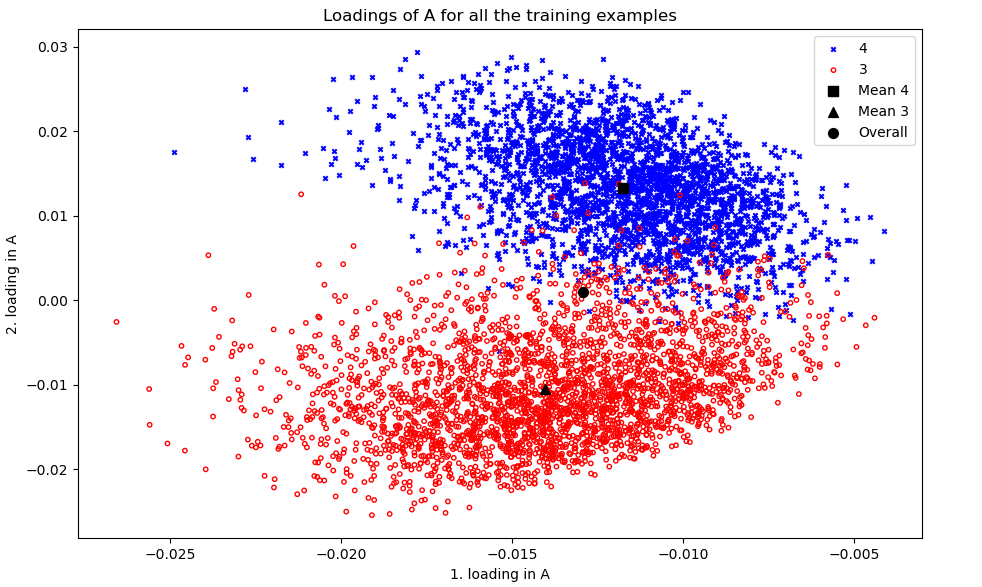
\includegraphics[width=\linewidth]{Pics/06_results/LoadingsOfAScatterMNIST.png}
        \caption{Scatter plot of the 2 loadings of the loading matrix $\bs{A}$ for the MNIST 3s and 4s respectively using rank 2 in the input dimension. The mean of the 2 clusters and overall is also marked with black.}
        \label{fig:loadingAMatrix}
    \end{subfigure}
    \begin{subfigure}{0.3\linewidth}
    \centering
        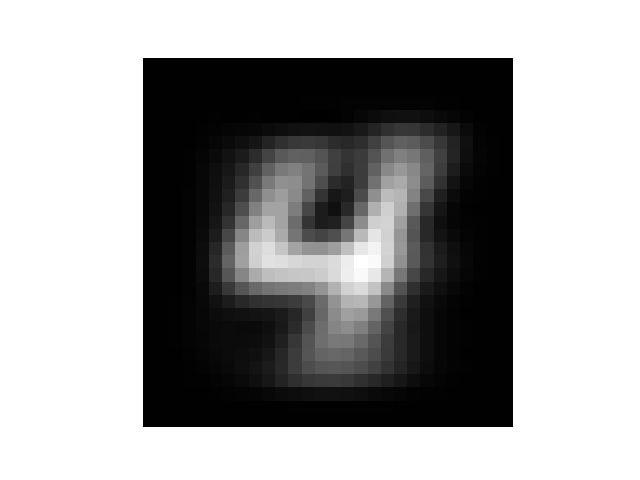
\includegraphics[width=.5\linewidth]{Pics/06_results/general4.png}
        \caption{The mean of 4s loadings}
    \end{subfigure}
    \begin{subfigure}{0.3\linewidth}
    \centering
        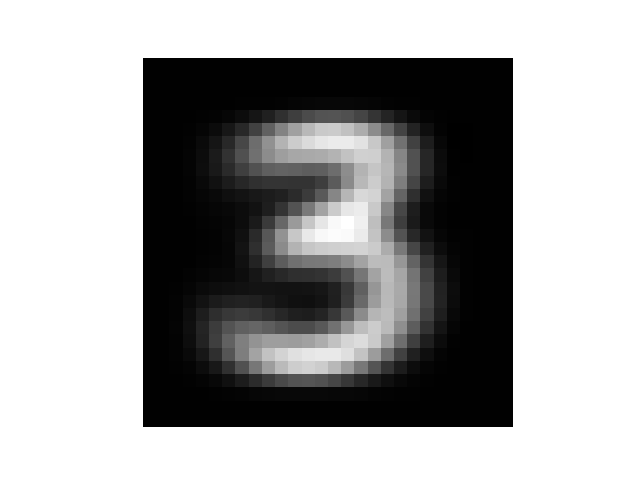
\includegraphics[width=.5\linewidth]{Pics/06_results/general3.png}
        \caption{The mean of 3s loadings}
    \end{subfigure}
    \begin{subfigure}{0.3\linewidth}
    \centering
        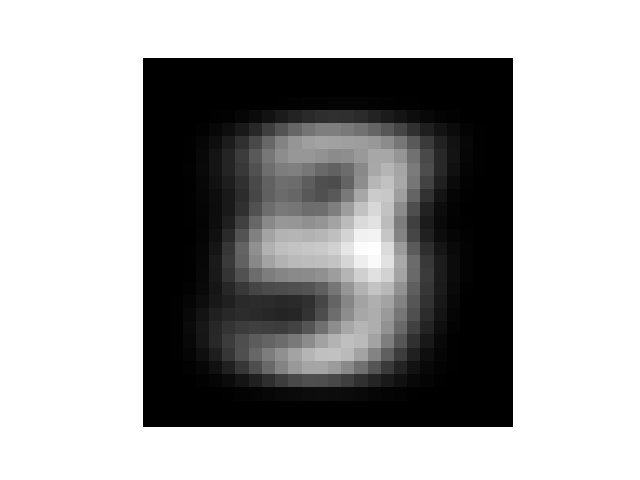
\includegraphics[width=.5\linewidth]{Pics/06_results/general.png}
        \caption{The mean of all loadings}
        \label{Hej}
    \end{subfigure}
    \caption{Scatter plot of the 2 loadings of $\bs{A}$ for the MNIST 3s and 4s using rank 2 including mean in each of the clusters and overall. Using these means as loadings in the approximation gives the approximated "general" 3, 4 and overall given in \textbf{(b)-(d)}. Notice how the overall mean gives a mixture of a 3 and a 4.}
    \label{fig:loadingsOfA}
\end{figure}

This all comes down to the loadings of $\bs{A}$ holding a great deal of information about which pictures are 3s and which are 4s. This information could be used as input into the NN instead of the actual pictures potentially reducing the number of parameters dramatically (from 784 to 2 input neurons in this example). 

\paragraph{Using THETIS forehand flat and backhand}
Following the same procedure as for the MNIST 3s and 4s we set the rank of the decomposition to 2. Stacking $N$ videos and decomposing with rank 2 in the between sample dimension yields:
\begin{equation}
    \tensor{X}^{N\times 4 \times 28 \times 120 \times 160} \approx \tensor{G}^{2 \times 4 \times 28 \times 120 \times 160} \times_1 \bs{A}^{N\times 2}
\end{equation}
Now the loading matrix $\bs{A}$ holds 2 values for each observation that should ideally be separating the two types of shots. Making the scatter plot of the loadings from $\bs{A}$ colored with the type this is however not the case. The plot is shown in XXX, where it is clear that there are two clusters, but the clusters does not separate the type of shot, but the setting of the video.
\begin{figure}
    \centering
    \includegraphics{}
    \caption{Caption}
    \label{fig:my_label}
\end{figure}